\section{Formulario complementario}
\begingroup
\footnotesize
\setlength{\parindent}{0pt}
\setlength{\abovedisplayskip}{3pt}
\setlength{\belowdisplayskip}{3pt}
\setlength{\abovedisplayshortskip}{3pt}
\setlength{\belowdisplayshortskip}{3pt}

\subsection*{Sistemas coordenados}
Convención: $r$ es la distancia al eje $z$, $\rho$ la distancia al origen,
$\theta$ el ángulo en $xy$ desde $+x$ y $\varphi$ el ángulo desde $+z$.
\[
r\geq0,\quad \rho\geq0,\quad 0\leq\theta<2\pi,\quad 0\leq\varphi\leq\pi.
\]
\begin{align*}
\text{Polares }(r,\theta):&\quad x=r\cos\theta,\quad y=r\sin\theta,\\
\text{Cilíndricas }(r,\theta,z):&\quad x=r\cos\theta,\quad y=r\sin\theta,\quad z=z,\\
\text{Esféricas }(\rho,\theta,\varphi):&\quad
x=\rho\sin\varphi\cos\theta,\quad y=\rho\sin\varphi\sin\theta,\quad z=\rho\cos\varphi.
\end{align*}
Conversiones inversas y relación entre radios:
\[
r=\sqrt{x^2+y^2},\qquad \rho=\sqrt{x^2+y^2+z^2},\qquad
r=\rho\sin\varphi,\quad z=\rho\cos\varphi.
\]
\[
\theta=\operatorname{atan2}(y,x)\pmod{2\pi}\quad(r>0),\qquad
\varphi=\arccos\frac{z}{\rho}\quad(\rho>0).
\]
$\operatorname{atan2}$ determina el cuadrante. Sobre el eje $z$, $\theta$ es
indeterminado; en el origen ambos ángulos esféricos son indeterminados.

\begin{center}
\begingroup\shorthandoff{>}
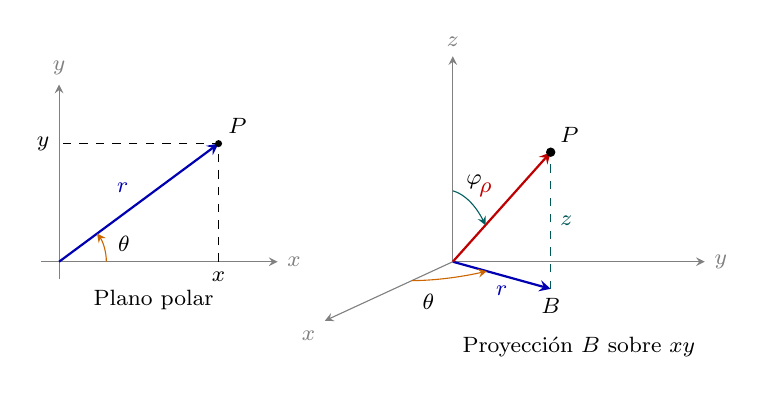
\begin{tikzpicture}[>=stealth,every node/.style={font=\footnotesize}]
\begin{scope}[scale=.75]
\draw[->,gray] (-.3,0)--(3.7,0) node[right] {$x$};
\draw[->,gray] (0,-.3)--(0,3) node[above] {$y$};
\draw[->,blue!70!black,thick] (0,0)--(2.7,2) node[midway,above left] {$r$};
\draw[dashed] (2.7,0)--(2.7,2)--(0,2);
\draw[->,orange!80!black] (.8,0) arc(0:36.53:.8);
\node at (1.1,.3) {$\theta$};
\fill (2.7,2) circle (1.7pt) node[above right] {$P$};
\node[below] at (2.7,0) {$x$};\node[left] at (0,2) {$y$};
\node at (1.6,-.65) {Plano polar};
\end{scope}
\begin{scope}[shift={(5,0)},x={(-.65cm,-.3cm)},y={(1cm,0cm)},z={(0cm,.9cm)}]
\draw[->,gray] (0,0,0)--(2.5,0,0) node[below left] {$x$};
\draw[->,gray] (0,0,0)--(0,3.2,0) node[right] {$y$};
\draw[->,gray] (0,0,0)--(0,0,2.9) node[above] {$z$};
% P tiene rho=3, theta=60 grados y phi=50 grados.
\coordinate (B) at (1.1491,1.9902,0);
\coordinate (P) at (1.1491,1.9902,1.9284);
\draw[->,blue!70!black,thick] (0,0,0)--(B) node[midway,below] {$r$};
\draw[dashed,teal!70!black] (B)--(P) node[midway,right] {$z$};
\draw[->,red!75!black,thick] (0,0,0)--(P) node[midway,above left] {$\rho$};
\draw[->,orange!80!black] plot[domain=0:60,samples=20]
 ({.8*cos(\x)},{.8*sin(\x)},0);
\node at (1.4,.6,-.1) {$\theta$};
\draw[->,teal!75!black] plot[domain=0:50,samples=20]
 ({sin(\x)*cos(60)},{sin(\x)*sin(60)},{cos(\x)});
\node at (.2,.4,1.2) {$\varphi$};
\fill (P) circle (1.7pt) node[above right] {$P$};
\node[below] at (B) {$B$};
\node at (0,1.6,-1.2) {Proyección $B$ sobre $xy$};
\end{scope}
\end{tikzpicture}
\endgroup
\end{center}

\subsection*{Superficies coordenadas y elementos de integración}
\renewcommand{\arraystretch}{1.5}
\begin{center}
\begin{tabular}{lll}
\hline
Sistema & Coordenada constante & Superficie\\\hline
Cilíndricas & $r=a>0$ & Cilindro circular\\
 & $\theta=\theta_0$ & Semiplano vertical\\
 & $z=c$ & Plano horizontal\\
Esféricas & $\rho=a>0$ & Esfera\\
 & $\theta=\theta_0$ & Semiplano vertical\\
 & $\varphi=\varphi_0$, $0<\varphi_0<\pi/2$ & Semicono superior\\
 & $\varphi=\pi/2$ & Plano $xy$\\
 & $\varphi=\varphi_0$, $\pi/2<\varphi_0<\pi$ & Semicono inferior\\\hline
\end{tabular}
\end{center}
\[
\text{Polares: }dA=r\,dr\,d\theta,\quad
\text{Cilíndricas: }dV=r\,dr\,d\theta\,dz,\quad
\text{Esféricas: }dV=\rho^2\sin\varphi\,d\rho\,d\varphi\,d\theta.
\]
En $\varphi=0,\pi$ las superficies coordenadas se reducen a semiejes.
Los factores anteriores son valores absolutos de jacobianos.

\newpage
\subsection*{Notación de índices y suma de Einstein}
Se usan coordenadas cartesianas ortonormales con orientación de mano derecha:
$(x_1,x_2,x_3)=(x,y,z)$, índices en $\{1,2,3\}$ y $\partial_i=\partial/\partial x_i$.
Un índice repetido dos veces se suma; un índice libre identifica la componente.
\[
a_ib_i=\sum_{i=1}^3a_ib_i,\qquad
A_{ij}b_j=\sum_{j=1}^3A_{ij}b_j=c_i,\qquad
A_{ij}b_j=A_{ik}b_k.
\]
Los índices libres coinciden en todos los términos de una igualdad.
Un mismo índice no aparece más de dos veces en un producto.

\subsection*{Delta de Kronecker y símbolo de Levi-Civita}
\[
\delta_{ij}=\begin{cases}1,&i=j,\\0,&i\ne j,\end{cases}\qquad
\varepsilon_{ijk}=\begin{cases}
+1,&(i,j,k)=(1,2,3),(2,3,1),(3,1,2),\\
-1,&(i,j,k)=(1,3,2),(3,2,1),(2,1,3),\\
0,&\text{algún índice se repite}.
\end{cases}
\]
\[
\delta_{ij}a_j=a_i,\quad \delta_{ij}\delta_{jk}=\delta_{ik},\quad
\delta_{ii}=3,\quad \partial_i x_j=\delta_{ij},\quad \partial_i x_i=3.
\]
\[
\varepsilon_{ijk}=\varepsilon_{jki}=\varepsilon_{kij},\qquad
\varepsilon_{ijk}=-\varepsilon_{jik}=-\varepsilon_{ikj}.
\]
\[
\varepsilon_{ijk}\varepsilon_{ilm}=\delta_{jl}\delta_{km}-\delta_{jm}\delta_{kl},
\qquad \varepsilon_{ijk}\varepsilon_{ijl}=2\delta_{kl},\qquad
\varepsilon_{ijk}\varepsilon_{ijk}=6.
\]
\[
S_{ij}=S_{ji},\quad A_{ij}=-A_{ji}\quad\Longrightarrow\quad S_{ij}A_{ij}=0.
\]

\subsection*{Operaciones vectoriales y operadores diferenciales}
\begin{align*}
\mathbf a\cdot\mathbf b&=a_ib_i,&
(\mathbf a\times\mathbf b)_i&=\varepsilon_{ijk}a_jb_k,\\
(\nabla f)_i&=\partial_i f,&
\nabla\cdot\mathbf F&=\partial_iF_i,\\
(\nabla\times\mathbf F)_i&=\varepsilon_{ijk}\partial_jF_k,&
\nabla^2f&=\partial_i\partial_i f=f_{xx}+f_{yy}+f_{zz}.
\end{align*}
El laplaciano vectorial se aplica por componentes:
$(\nabla^2\mathbf F)_i=\partial_j\partial_jF_i$.
\[
\partial_i(fg)=(\partial_i f)g+f\partial_i g,\qquad
\partial_i\partial_jf=\partial_j\partial_if\quad(f\in C^2).
\]

\subsection*{Identidades vectoriales}
Para campos de clase $C^1$ en las identidades de primer orden y de clase $C^2$
en las de segundo orden:
\begin{align*}
\nabla\cdot(f\mathbf F)&=\nabla f\cdot\mathbf F+f\nabla\cdot\mathbf F,\\
\nabla\times(f\mathbf F)&=\nabla f\times\mathbf F+f\nabla\times\mathbf F,\\
\nabla\cdot(\mathbf F\times\mathbf G)&=\mathbf G\cdot(\nabla\times\mathbf F)
-\mathbf F\cdot(\nabla\times\mathbf G),\\
\nabla\times\nabla f&=\mathbf0,\qquad \nabla\cdot(\nabla\times\mathbf F)=0,\\
\nabla\times(\nabla\times\mathbf F)&=\nabla(\nabla\cdot\mathbf F)-\nabla^2\mathbf F,\\
\mathbf a\times(\mathbf b\times\mathbf c)&=\mathbf b(\mathbf a\cdot\mathbf c)-\mathbf c(\mathbf a\cdot\mathbf b),\\
(\mathbf a\times\mathbf b)\cdot(\mathbf c\times\mathbf d)
&=(\mathbf a\cdot\mathbf c)(\mathbf b\cdot\mathbf d)-(\mathbf a\cdot\mathbf d)(\mathbf b\cdot\mathbf c),\\
\|\mathbf a\times\mathbf b\|^2&=\|\mathbf a\|^2\|\mathbf b\|^2-(\mathbf a\cdot\mathbf b)^2.
\end{align*}
Campo conservativo: $\mathbf F=\nabla\psi$.
Si $\mathbf F\in C^1$ en un dominio abierto y simplemente conexo,
$\nabla\times\mathbf F=\mathbf0$ equivale a que $\mathbf F$ sea conservativo.
\endgroup
